\section{Reazione a catena della polimerasi -- PCR}

\subsection{Materiali e composti utilizzati}
\paragraph{Strumentazione}
\begin{itemize}[person]
	\itemb[Termociclatore:] strumento che viene utilizzatore per la PCR. È costituito da una griglia, dove vengano appoggiate le provette, che si scalda a temperature diverse a seconda della fase del ciclo di replicazione mentre il coperchio possiede una temperatura maggiore per evitare che la soluzione evapori.
	I cicli di riscaldamento, per il protocollo attuale, sono i seguenti:
	\begin{itemize}[squareItem]
		\itemb[Denaturazione iniziale:] \qty{3}{\min} a \qty{95}{\celsius}
		\itemb[Amplificazione] per 35 cicli, ogni ciclo si divide in:
		\begin{itemize}[squareItem]
			\itemb[Denaturazione]: \qty{30}{\sec} a \qty{95}{\celsius}
			\itemb[Ibridazione]: \qty{30}{\sec} a \qty{55}{\celsius}
			\itemb[Estensione]: \qty{60}{\sec} a \qty{72}{\celsius}
		\end{itemize}
		\itemb[Estensione finale:] \qty{5}{\min} a \qty{72}{\celsius}
	\end{itemize}
\end{itemize}

\paragraph{Composti utilizzati}
\begin{itemize}
	\itemb[Buffer TAQ (10X):] buffer necessario per mantenere il \pH\ stabile e per costituire l'ambiente adatto alla reazione
	\itemb[\ch{MgCl2}]: gli ioni magnesio \ch{Mg^2+} sono il cofattore della TAQ polimerasi
	\itemb[Primer FOR]: denominato \foreignlanguage{english}{forward} in quanto è complementare al filamento \(3' \rightarrow 5'\)
	\itemb[Primer REV]: denominato \foreignlanguage{english}{reverse} in quanto è complementare al filamento \(3' \rightarrow 5'\)
	\itemb[dNTPs]: sono i nucleotidi che devono essere polimerizzati
	\itemb[DNA plasmidico contenente l'inserto da amplificare (GPR3), circa 1000 basi]
	\itemb[\enzima{TAQ polimerasi}]: denominata anche \enzima{DNA polimerasi termostabile} perché la sua temperatura ottimale è di \qtyrange{75}{80}{\celsius}. Viene utilizzata nella PCR per questa sua caratteristica, in quanto per far si che il DNA venga amplificato è necessaria una temperatura di \qty{94}{\celsius}
\end{itemize}

\subsection{Protocollo}
\subsubsection{Preparazione ed esecuzione della PCR }
\begin{enumerate}
	\item In una Eppendorf da \qty{250}{\micro\litre} aggiungere:
	      \begin{itemize}[person]
		      \item \qty{12.5}{\micro\litre} di \ch{H2O} sterile
		      \item \qty{2}{\micro\litre} di buffer TAQ (10X)
		      \item \qty{1}{\micro\litre} di \ch{MgCl2} \qty{50}{\milli\Molar}
		      \item \qty{1}{\micro\litre} di primer FOR \qty{25}{\milli\Molar}
		      \item \qty{1}{\micro\litre} di primer REV \qty{25}{\milli\Molar}
		      \item \qty{1}{\micro\litre} di dNTPs \qty{10}{\milli\Molar}
		      \item \qty{1}{\micro\litre} di DNA plasmidico
		      \item \qty{0.5}{\micro\litre} di TAQ polimerasi
	      \end{itemize}
	      In totale avremo una soluzione di \qty{20}{\micro\litre}
	\item Inserire la soluzione nel termociclatore e avviare la PCR
	\item Una volta finiti tutti i cicli della PCR, tenere a \qty{12}{\celsius} il campione fin quando non lo si recupera
	\item Preparare il gel di agarosio (la preparazione del gel è descritta in \ref{sssec:agarosio})
	\item Inserire il campione nel gel e far partire l'elettroferesi
\end{enumerate}

% \subsubsection{Preparazione del gel di agarosio}
% \begin{enumerate}
% 	\item Preparare il gel di agarosio \qty{0.8}{\percent} mediante:
% 	\begin{itemize}[person]
% 		\item \qty{0.6}{\g} di agarosio
% 		\item \qty{1.6}{\ml} di TAE 50X
% 		\item \qty{78.4}{\ml} di \ch{H2O}
% 	\end{itemize}
% 	\item Scaldare il composto nella beuta per far sciogliere l'agarosio
% 	\item Aspettare qualche minuto per far raffreddare
% 	\item Aggiungere \qty{4}{\micro\litre} di SyberSafe e versare il composto nella vaschetta precedentemente preparata
% 	\item Rimuovere il pettinino e inserire il gel solidificato nella vaschetta di corsa
% 	\item Coprire con \qty{250}{\ml} di buffer di corsa (TAE 1X)
% \end{enumerate}

Per verificare che la PCR sia venuta con successo, prima di tutto, far correre il campione sottoposto a PCR sul gel di agarosio e poi guardare agli UV il gel. Se la PCR è venuta con successo sarà presente una banda unica (\hyperref[img:4-01]{Fig.~\ref{img:4-01}.C}) altrimenti non si presenterà nessuna banda. L'insuccesso della procedura può essere rimandata alla non aggiunta di una delle componenti della soluzione iniziale, durante la sua preparazione (\hyperref[img:4-01]{Fig.~\ref{img:4-01}.B}).

\begin{minipage}{0.7\textwidth}
	\begin{figure}[H]
		\captionsetup{singlelinecheck=off}
		\centering
		\begin{annotatedFigure}
			{
				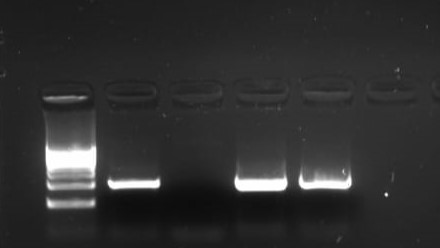
\includegraphics[scale=.8]{4-01}
			}
			\annotatedFigureText{0.16,0.75}{black}{font={\sffamily\small},inner sep=2pt}{A}
			\annotatedFigureText{0.45,0.75}{black}{font={\sffamily\small},inner sep=2pt}{B}
			\annotatedFigureText{0.6,0.75}{black}{font={\sffamily\small},inner sep=2pt}{C}
		\end{annotatedFigure}
		\caption{\\Campioni sottoposti a PCR\\ su gel di agarosio visti agli UV}\label{img:4-01}
	\end{figure}
\end{minipage}
\begin{minipage}[b]{0.25\textwidth}
	\begin{enumerate}[label=\Alph*)]
		\item Marker
		\item PCR avvenuta con insuccesso
		\item PCR avvenuta con successo
	\end{enumerate}
\end{minipage}